\section{Resultados}

\begin{longtable}{|c|c|c|c|c|c|c|c|}
    \hline
    \rowcolor{azulito}\multicolumn{8}{|c|}{Cono 1} \\
    \hline
    \rowcolor{azulito} $t_{1/2}$ (s) & $v_{1/2}$ (m/s) & $f_{1/2} $ (N)& $t$ (s)& $y$ (m)& $v$ (m/s)& $f$ (N)& $a$ (m/$s^2$)\\
    \endhead
    \hline 0.0165 & -0.1617 & -0.0151 & 0 & 2.000 & 0.00000 & -0.0154 & -9.80 \\
    \hline 0.0495 & -0.4649 & -0.0133 & 0.033 & 1.995 & -0.31818 & -0.0144 & -9.19 \\
    \hline 0.0825 & -0.7168 & -0.0105 & 0.066 & 1.979 & -0.59842 & -0.0120 & -7.63 \\
    \hline 0.1155 & -0.9062 & -0.0076 & 0.099 & 1.956 & -0.81923 & -0.0090 & -5.74 \\
    \hline 0.1485 & -1.0383 & -0.0051 & 0.132 & 1.926 & -0.97867 & -0.0063 & -4.00 \\
    \hline 0.1815 & -1.1259 & -0.0033 & 0.165 & 1.892 & -1.08680 & -0.0042 & -2.65 \\
    \hline 0.2145 & -1.1819 & -0.0021 & 0.198 & 1.854 & -1.15709 & -0.0027 & -1.70 \\
    \hline 0.2475 & -1.2170 & -0.0013 & 0.231 & 1.815 & -1.20155 & -0.0017 & -1.06 \\
    \hline 0.2805 & -1.2387 & -0.0008 & 0.264 & 1.775 & -1.22919 & -0.0010 & -0.66 \\
    \hline 0.3135 & -1.2520 & -0.0005 & 0.297 & 1.734 & -1.24619 & -0.0006 & -0.40 \\
    \hline 0.3465 & -1.2601 & -0.0003 & 0.33 & 1.693 & -1.25658 & -0.0004 & -0.25 \\
    \hline 0.3795 & -1.2651 & -0.0002 & 0.363 & 1.651 & -1.26290 & -0.0002 & -0.15 \\
    \hline 0.4125 & -1.2680 & -0.0001 & 0.396 & 1.610 & -1.26673 & -0.0001 & -0.09 \\
    \hline 0.4455 & -1.2699 & -0.0001 & 0.429 & 1.568 & -1.26906 & -0.0001 & -0.05 \\
    \hline 0.4785 & -1.2709 & 0.0000 & 0.462 & 1.526 & -1.27047 & -0.0001 & -0.03 \\
    \hline 0.5115 & -1.2716 & 0.0000 & 0.495 & 1.484 & -1.27132 & 0.0000 & -0.02 \\
    \hline 0.5445 & -1.2720 & 0.0000 & 0.528 & 1.442 & -1.27184 & 0.0000 & -0.01 \\
    \hline 0.5775 & -1.2723 & 0.0000 & 0.561 & 1.400 & -1.27215 & 0.0000 & -0.01 \\
    \hline 0.6105 & -1.2724 & 0.0000 & 0.594 & 1.358 & -1.27234 & 0.0000 & 0.00 \\
    \hline
    \caption{Solución con el método numérico
    para la primer cono.}
    \label{tab:Cono1Euler}
\end{longtable}
    \clearpage
\begin{longtable}{|c|c|c|c|c|c|c|c|}
    \hline
    \rowcolor{azulito}\multicolumn{8}{|c|}{Cono 2} \\
    \hline
    \rowcolor{azulito} $t_{1/2}$ (s) & $v_{1/2}$ (m/s) & $f_{1/2} $ (N)& $t$ (s)& $y$ (m)& $v$ (m/s)& $f$ (N)& $a$ (m/$s^2$)\\
    \endhead
    \hline 0.0165 & -0.1617 & -0.0200 & 0.000 & 2.000 & 0.0000 & -0.0203 & -9.80 \\
    \hline 0.0495 & -0.4696 & -0.0182 & 0.033 & 1.995 & -0.3194 & -0.0193 & -9.33 \\
    \hline 0.0825 & -0.7368 & -0.0151 & 0.066 & 1.979 & -0.6094 & -0.0168 & -8.10 \\
    \hline 0.1155 & -0.9506 & -0.0117 & 0.099 & 1.955 & -0.8506 & -0.0134 & -6.48 \\
    \hline 0.1485 & -1.1111 & -0.0086 & 0.132 & 1.923 & -1.0372 & -0.0101 & -4.86 \\
    \hline 0.1815 & -1.2259 & -0.0060 & 0.165 & 1.887 & -1.1736 & -0.0072 & -3.48 \\
    \hline 0.2145 & -1.3053 & -0.0041 & 0.198 & 1.846 & -1.2694 & -0.0050 & -2.41 \\
    \hline 0.2475 & -1.3589 & -0.0027 & 0.231 & 1.803 & -1.3348 & -0.0034 & -1.62 \\
    \hline 0.2805 & -1.3945 & -0.0018 & 0.264 & 1.758 & -1.3785 & -0.0022 & -1.08 \\
    \hline 0.3135 & -1.4179 & -0.0012 & 0.297 & 1.712 & -1.4074 & -0.0015 & -0.71 \\
    \hline 0.3465 & -1.4332 & -0.0008 & 0.330 & 1.666 & -1.4263 & -0.0010 & -0.46 \\
    \hline 0.3795 & -1.4431 & -0.0005 & 0.363 & 1.618 & -1.4387 & -0.0006 & -0.30 \\
    \hline 0.4125 & -1.4495 & -0.0003 & 0.396 & 1.571 & -1.4467 & -0.0004 & -0.20 \\
    \hline 0.4455 & -1.4537 & -0.0002 & 0.429 & 1.523 & -1.4518 & -0.0003 & -0.13 \\
    \hline 0.4785 & -1.4564 & -0.0001 & 0.462 & 1.475 & -1.4552 & -0.0002 & -0.08 \\
    \hline 0.5115 & -1.4581 & -0.0001 & 0.495 & 1.427 & -1.4574 & -0.0001 & -0.05 \\
    \hline 0.5445 & -1.4593 & -0.0001 & 0.528 & 1.379 & -1.4588 & -0.0001 & -0.03 \\
    \hline 0.5775 & -1.4600 & 0.0000 & 0.561 & 1.331 & -1.4597 & 0.0000 & -0.02 \\
    \hline 0.6105 & -1.4604 & 0.0000 & 0.594 & 1.282 & -1.4602 & 0.0000 & -0.01 \\
    \hline 0.6435 & -1.4607 & 0.0000 & 0.627 & 1.234 & -1.4606 & 0.0000 & -0.01 \\
    \hline 0.6765 & -1.4609 & 0.0000 & 0.660 & 1.186 & -1.4609 & 0.0000 & -0.01 \\
    \hline 0.7095 & -1.4611 & 0.0000 & 0.693 & 1.138 & -1.4610 & 0.0000 & 0.00 \\
    \hline
    \caption{Solución con el método numérico
    para la segunda cono.}
    \label{tab:Cono2Euler}
\end{longtable}
\begin{longtable}{|c|c|c|c|c|c|c|c|}
    \hline
    \rowcolor{azulito}\multicolumn{8}{|c|}{Cono 3} \\
    \hline
    \rowcolor{azulito} $t_{1/2}$ (s) & $v_{1/2}$ (m/s) & $f_{1/2} $ (N)& $t$ (s)& $y$ (m)& $v$ (m/s)& $f$ (N)& $a$ (m/$s^2$)\\
    \endhead
    \hline 0.0165 & -0.1617 & -0.0249 & 0.000 & 2.000 & 0.0000 & -0.0252 & -9.80 \\
    \hline 0.0495 & -0.4726 & -0.0231 & 0.033 & 1.995 & -0.3202 & -0.0242 & -9.42 \\
    \hline 0.0825 & -0.7496 & -0.0198 & 0.066 & 1.979 & -0.6164 & -0.0216 & -8.40 \\
    \hline 0.1155 & -0.9805 & -0.0161 & 0.099 & 1.954 & -0.8712 & -0.0180 & -6.99 \\
    \hline 0.1485 & -1.1623 & -0.0124 & 0.132 & 1.922 & -1.0773 & -0.0142 & -5.51 \\
    \hline 0.1815 & -1.2993 & -0.0091 & 0.165 & 1.884 & -1.2360 & -0.0107 & -4.15 \\
    \hline 0.2145 & -1.3993 & -0.0066 & 0.198 & 1.841 & -1.3534 & -0.0078 & -3.03 \\
    \hline 0.2475 & -1.4705 & -0.0046 & 0.231 & 1.795 & -1.4380 & -0.0055 & -2.16 \\
    \hline 0.2805 & -1.5203 & -0.0032 & 0.264 & 1.746 & -1.4976 & -0.0039 & -1.51 \\
    \hline 0.3135 & -1.5547 & -0.0022 & 0.297 & 1.696 & -1.5391 & -0.0027 & -1.04 \\
    \hline 0.3465 & -1.5783 & -0.0015 & 0.330 & 1.645 & -1.5676 & -0.0018 & -0.72 \\
    \hline 0.3795 & -1.5944 & -0.0010 & 0.363 & 1.592 & -1.5872 & -0.0013 & -0.49 \\
    \hline 0.4125 & -1.6054 & -0.0007 & 0.396 & 1.540 & -1.6004 & -0.0009 & -0.33 \\
    \hline 0.4455 & -1.6128 & -0.0005 & 0.429 & 1.487 & -1.6095 & -0.0006 & -0.22 \\
    \hline 0.4785 & -1.6178 & -0.0003 & 0.462 & 1.434 & -1.6156 & -0.0004 & -0.15 \\
    \hline 0.5115 & -1.6212 & -0.0002 & 0.495 & 1.380 & -1.6197 & -0.0003 & -0.10 \\
    \hline 0.5445 & -1.6235 & -0.0001 & 0.528 & 1.327 & -1.6225 & -0.0002 & -0.07 \\
    \hline 0.5775 & -1.6250 & -0.0001 & 0.561 & 1.273 & -1.6243 & -0.0001 & -0.05 \\
    \hline 0.6105 & -1.6261 & -0.0001 & 0.594 & 1.220 & -1.6256 & -0.0001 & -0.03 \\
    \hline 0.6435 & -1.6268 & 0.0000 & 0.627 & 1.166 & -1.6265 & -0.0001 & -0.02 \\
    \hline 0.6765 & -1.6273 & 0.0000 & 0.660 & 1.112 & -1.6270 & 0.0000 & -0.01 \\
    \hline 0.7095 & -1.6276 & 0.0000 & 0.693 & 1.059 & -1.6274 & 0.0000 & -0.01 \\
    \hline 0.7425 & -1.6278 & 0.0000 & 0.726 & 1.005 & -1.6277 & 0.0000 & -0.01 \\
    \hline 0.7755 & -1.6279 & 0.0000 & 0.759 & 0.951 & -1.6279 & 0.0000 & 0.00 \\
    \hline
    \caption{Solución numerica para el tercer cono.}
    \label{tab:Cono3}
\end{longtable}

Para conocer la discrepancia porcentual se ocupa la siguiente expresión:

\begin{equation}
    \left( y - y_M \right)^2
    \label{Discrepacnai}
\end{equation}

Y se obtienen los siguientes resultados:

\begin{table}[h]
    \centering
    \begin{tabular}{|c|c|c|}
        \hline
        \rowcolor{azulito} Cono & Discrepancia \\
%         \hline 1    & 0.049218615 \\
%         \hline 2    & 0.034303902 \\
%         \hline 3    & 0.044536735 \\
        \hline 1    & 0.0492 \\
        \hline 2    & 0.0343 \\
        \hline 3    & 0.0445 \\
        \hline
    \end{tabular}
    \caption{Valores obtenidos con la expresión \ref{Discrepacnai} de cada cono.}
    \label{tab:Discrepancias}
\end{table}

\begin{figure}[h!]
    \centering
    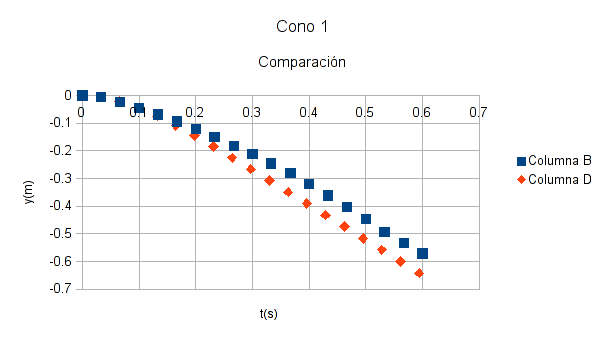
\includegraphics{cono1}
    \caption{Gráfica comparativa de los datos obtenidos entre el método
    numérico y los experimentales.}
    \label{fig:Cono1}
\end{figure}

\begin{figure}[h!]
    \centering
    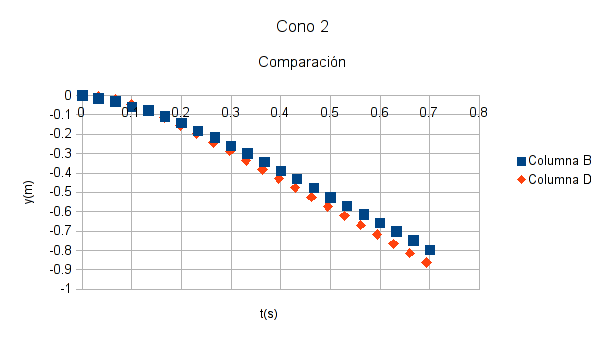
\includegraphics{cono2}
    \caption{Gráfica comparativa de los datos obtenidos entre el método
    numérico y los experimentales.}
    \label{fig:Cono2}
\end{figure}

\begin{figure}[h!]
    \centering
    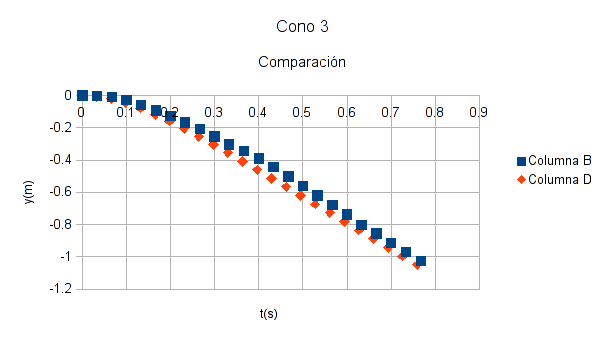
\includegraphics{cono3}
    \caption{Gráfica comparativa de los datos obtenidos entre el método
    numérico y los experimentales.}
    \label{fig:Cono3}
\end{figure}
